\documentclass{exam}
\usepackage{tasks}

\usepackage{amsmath,amssymb,amsfonts}
\usepackage{graphicx}
\usepackage{amsthm}
\usepackage[french]{babel}
\usepackage{enumitem}
\pagestyle{empty}
\graphicspath{ {../Images/} }

\usepackage{geometry}
\geometry{left=1.5cm, right=1.5cm, top=1.5cm, bottom=1.5cm}


%\setlength{\topmargin}{-.5in} \setlength{\textheight}{9.25in}
%\setlength{\oddsidemargin}{0in} \setlength{\textwidth}{6.8in}

\makeatletter
\def\gap#1{%
  \setbox\@tempboxa\hbox{{\color{white}#1}}%
  \@tempdima\wd\@tempboxa
  \rlap{\unhbox\@tempboxa}%
  \hb@xt@\@tempdima{\dotfill}%
}
\makeatother   

\theoremstyle{definition}
\newtheorem{exercice}{Exercice}

\begin{document}
\large

\noindent{\bf Contrôle 3 (D) -- 55min. \hfill Première générale \hfill 20/11/2024}

% \vspace{2mm}
% 
% \noindent{\makebox[\textwidth]{Nom et prénom:\enspace\hrulefill}}
% 
% \vspace{2mm}

% \begin{exercice}{(10 min}
%     Donner, lorsqu'elle existe, la forme factorisée des polynômes ci-dessous.
%     \begin{tasks}(2)
%         \task $-2x^2 + 7x - 3$. % 2 racines discriminant.
%         %\task $6x^2 - 6x + \dfrac{3}{2}$. % 1 racine
%         \task $-2x^2 +x - 1$. % pas de racines
%     \end{tasks}
% \end{exercice}

\begin{exercice}{(5 min)}
    Résoudre l'inéquation $152x^2 -54x - 98 \geq 0$.%suivantes :
    %Résoudre l'inéquation $2x^2 -5x + 3 \geq 0$.%suivantes :
    %\begin{tasks}(2)
    %    \task $3x^2 -5x + 2 \geq 0$. % 1 racine évidente
    %    %\task $-2x^2 -4x > 0$. % facteur évident
    %  245  %\task $x^2 - 6x + 9 > 0$. % ineq 1 racine
    %\end{tasks}
\end{exercice}

\begin{exercice}{(5 min)}
    Déterminer deux entiers naturels séparés de 2 nombres (par exemple $1$ et $3$) dont le produit est égal à $273528$.
    %Déterminez deux entiers naturels successifs dont le produit est égal à $46440$.
\end{exercice}

% \begin{exercice}
%     Soit $m \in \mathbb{R}$. On considère l'équation $x^2 + mx - m+3 = 0$. Pour quelles valeurs de $m$ l'équation admet-t'elle une unique solution ?
%     %Soit $m \in \mathbb{R}$. On considère l'équation $x^2 - mx - m+2 = 0$. Pour quelles valeurs de $m$ l'équation admet-t'elle une unique solution ?
% \end{exercice}

\begin{exercice}{(15 min)}
    Soit $a, b, c$ des réels non nuls et $f(x) = ax^2+bx+c$. On a représenté ci-dessous la parabole $\mathcal{C}_f$ représentant $f$:
    
    \begin{center}
        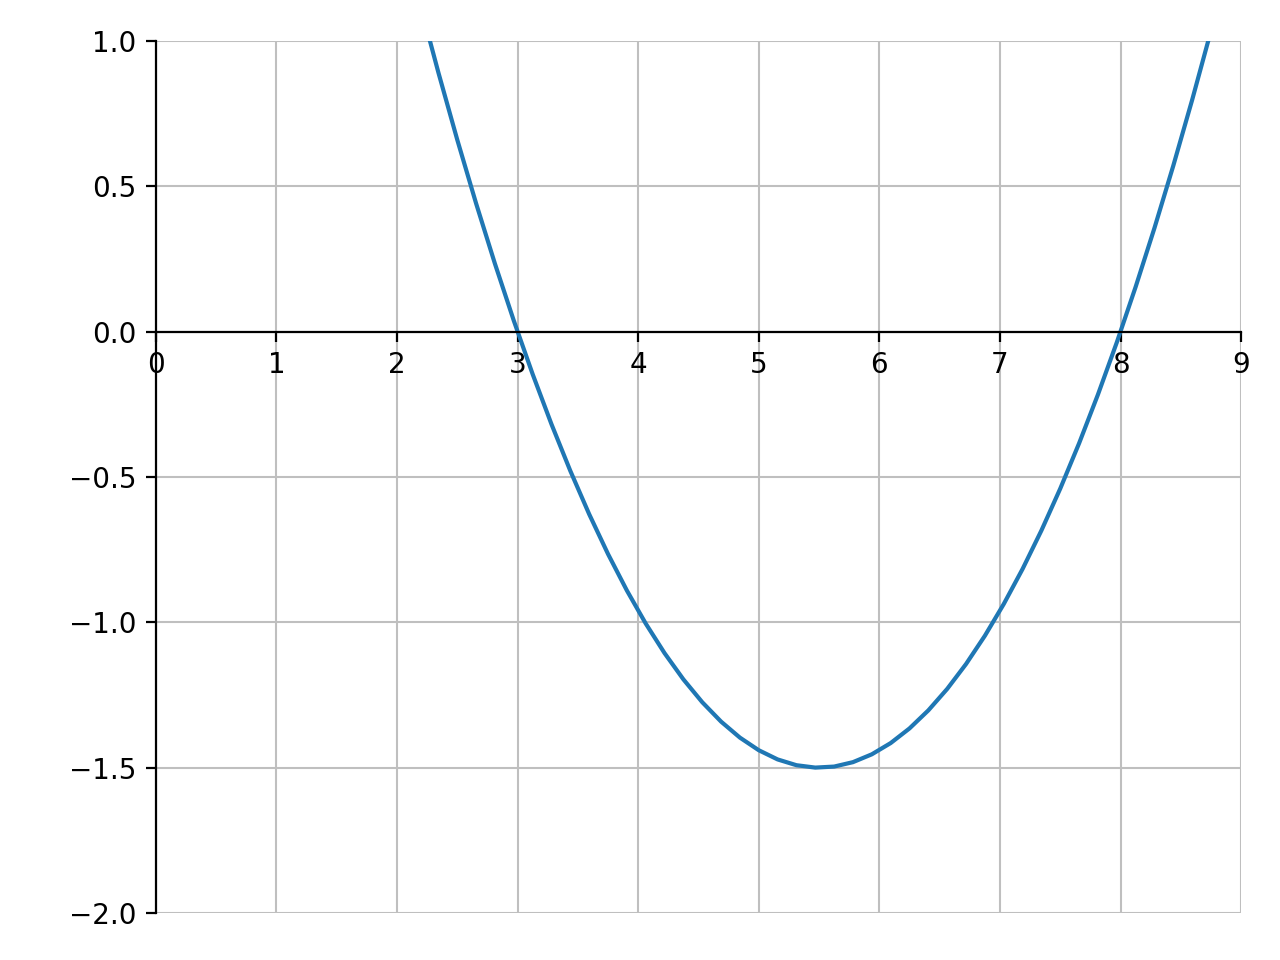
\includegraphics[width=0.6\linewidth]{functionD.png}
        %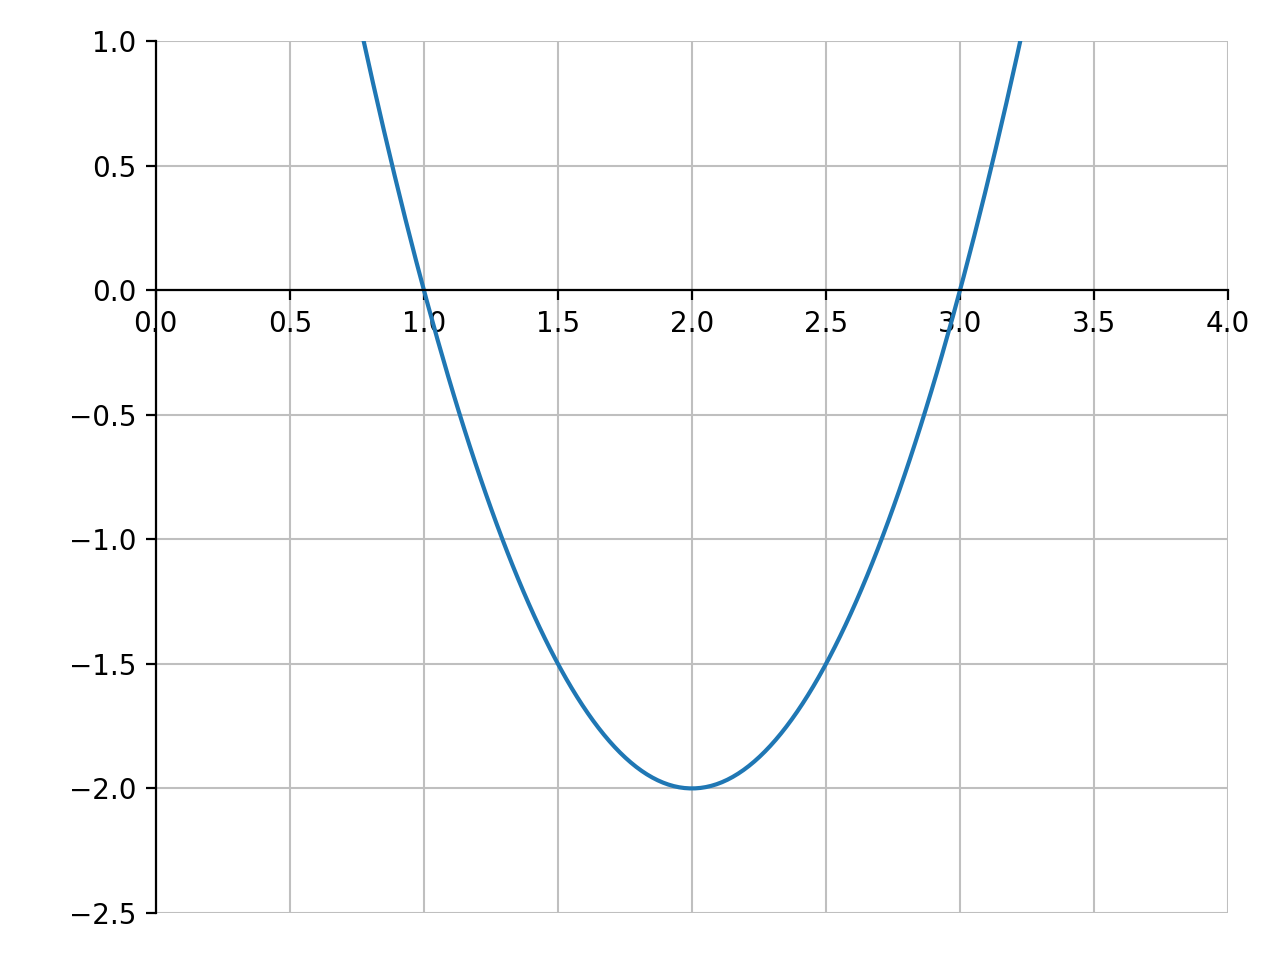
\includegraphics[width=0.6\linewidth]{functionB.png}
    \end{center}

    \begin{enumerate}
        \item \begin{enumerate}
            \item Donner les racines de $f$.
            \item Retrouver la valeur de $a$\footnote{Indice: il faut poser une équation utilisant des valeurs spécifiques pour $x$ et $f(x)$.}.
            \item En déduire la forme factorisée de $f$.
        \end{enumerate}
        \item \begin{enumerate}
            \item Donner les coordonnées du sommet de la parabole $\mathcal{C}_f$
            \item En utilisant les questions (1.b) et (2.a), déduire la forme canonique de $f$.
        \end{enumerate}
    \end{enumerate}
\end{exercice}

\begin{exercice}{(10 min)}
    Donner l'unique polynôme de degré 2 passant par $A(0;\ 4), B(3;\ 3)$ et $C(-1;\ 3)$.
    %Donner l'unique polynôme de degré 2 passant par les points $A(0,4), B(1, 6)$ et $C(-2, 6)$.
\end{exercice}

\begin{exercice}{(20 min)}
Une entreprise commercialise des automobiles : chaque voiture doit être vendue 8 000 euros. Sa production $x$ peut varier entre 0 et 100 000 voitures. Suite à une étude réalisée, les coûts de production sont donnés par la formule suivante :
\[
C(x) = 50x^2 + 1\,500x + 60\,000
\]
%\[
%C(x) = 50q^2 - 1\,000q + 80\,000
%\]
($x$ exprimé en millier de voitures et $C(x)$ exprimé en millier d’euros).

%On appelle coût fixe le coût que supporte l’entreprise même si la production est nulle.

\begin{enumerate}
    %\item Quel est le coût fixe supporté par cette entreprise de construction automobile ?
    \item Déterminer la quantité à partir de laquelle le coût de production est supérieur à 200 000 000 €.
    \item À combien s’élève le chiffre d’affaires pour une telle production ?\footnote{Indice: le chiffre d'affaire est obtenu en multipliant le prix de vente par le nombre d'unités vendues.}
    \item Exprimer, en fonction de $x$, le chiffre d’affaires noté $CA(x)$, en millier d’euros.
    \item En déduire la fonction $B(x)$ qui donne les bénéfices réalisés par l’entreprise.
    \item Dans quel intervalle doit se situer la quantité de voitures produites pour réaliser un bénéfice ?
    \item Quel est le nombre d’automobiles à produire pour un bénéfice maximal et quel est ce bénéfice ?
\end{enumerate}
\end{exercice}    

\end{document}